% BEGIN (PARALLELISATION)
% ===========================================================================
\subsection{Overview}

Within a FLAME simulation, every agent only interacts with its environment via the reading and writing of messages to a collection of Message Boards. This makes the Message Board component an ideal candidate for enabling parallelism. 

Using distributable Message Boards, agents can be farmed out across multiple processing nodes and simulated in parallel while coherency of the simulation is maintained through the unified view of the distributed Boards.

\begin{figure}[h]
 \centering
  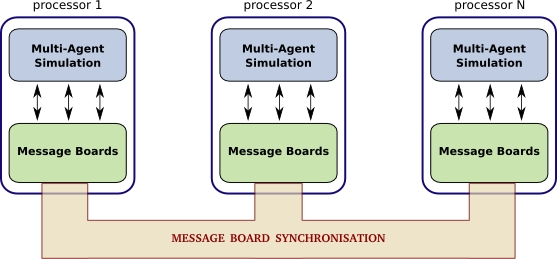
\includegraphics[scale=0.50]{mboard_flame.jpg}
 \caption{Parallelisation of FLAME using distributed Message Boards}
 \label{fig:mb_flame}
\end{figure}

\subsection{The Message Board library}
In the recent code release, the Message Board was decoupled from the FLAME framework and implemented as a separate library. This provides us with the flexibility to experiment with different parallelisation strategies while minimising the impact on current users of the FLAME framework.

\begin{figure}[h]
 \centering
  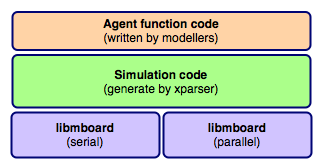
\includegraphics[scale=0.50]{mboard_overview.png}
 \caption{Users can create either serial or parallel executables by linking their object files to the appropriate \textit{libmboard} library}
 \label{fig:mb_overview}
\end{figure}

The Message Board Library (\textit{libmboard}) was built as a set of static libraries which can be linked to users' simulation object files to create serial and parallel executables. This setup enables users to maintain a common source base for both serial and parallel simulations, thus simplifying code management and testing. It will also provide \textit{libmboard} developers the facility to quickly switch between different library implementations without having to continuously recompile the test program.

All functionality provided by the Message Board Library is accessible via the \textit{libmboard} Application Program Interface (API). This is discussed further in Section~\ref{sec:mb_api}.

Within the FLAME framework, the \textit{libmboard} API is used within routines generated by the framework and not directly by the modellers. Modellers are provided with model-specific routines that hides to complexity of managing boards and packaging data into suitable datatypes. Figure~\ref{fig:mb_api_flame} provides and example of this whereby an agent's message add request gets translated to a \textit{libmboard} API call.
\begin{figure}[h]
 \centering
  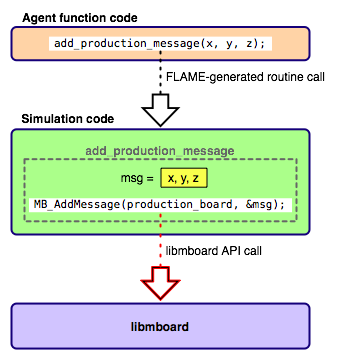
\includegraphics[scale=0.50]{mboard_codetranslate.png}
 \caption{Modellers use FLAME-generated routines which gets translated to the appropriate \textit{libmboard} API call}
 \label{fig:mb_api_flame}
\end{figure}

\textit{libmboard} uses MPI to communicate between processors, and POSIX threads (pthreads) to manage a separate thread for handling data management and inter-process communication. Futher details are available in Section~\ref{sec:mb_sync} and Section~\ref{sec:commthread}.

% ===========================================================================
\subsection{The \textit{libmboard} API}
\label{sec:mb_api}

\begin{itemize}
\item Quick desc of the API. Point to User Doc for details.
\item Opaque objects
\item return codes
\end{itemize} 


% ---------------------------------------------------------------------------
\subsubsection{Library environment}

\begin{itemize}
\item Init and finalise
\item MPI env
\item fork/join comm thread thread
\end{itemize} 

% ---------------------------------------------------------------------------
\subsubsection{Boards}

\begin{itemize}
\item create/clear/delete
\item AddMessage.. clone mem vs storing ptr
\end{itemize} 

% ---------------------------------------------------------------------------
\subsubsection{Iterators}

\begin{itemize}
\item isolate users from internal data representation
\item normal/filtered/sorted
\item returning cloned mem vs ptr.
\item randomisation
\item rewind
\end{itemize} 

% ---------------------------------------------------------------------------
\subsubsection{Synchronisation}
\label{sec:mb_sync}

\begin{itemize}
\item Message Tagging vs Filtered Iterators.
\item Why important? Impact on solution time?
\item Details on how messages are packed and distributed
\end{itemize} 

\begin{figure}[h]
 \centering
  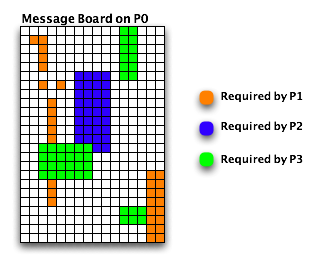
\includegraphics[scale=0.70]{taggedboard.png}
 \caption{Lorem ipsum dolor sit}
 \label{fig:taggedboard}
\end{figure}

When synchronisation of a board is requested, the board is locked and added into the \textit{Sync Queue}. Control is then returned to the the calling code, allowing it to perform other tasks that does not require access to the board being synchronised. 

The sequence diagram in  Figure~\ref{fig:syncboard} depicts how ra board synchronisation request may take place. The process of actually synchronising and unlocking the board is performed concurrently in the background by the \textit{Communication Thread}. This is discussed further in Section~\ref{sec:commthread}.

\begin{figure}[h]
 \centering
  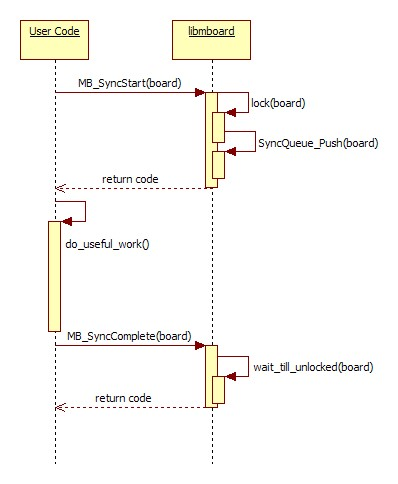
\includegraphics[scale=0.60]{syncboard.jpg}
 \caption{Other work can be schedule during board synchronisation to shadow the overheads of communication}
 \label{fig:syncboard}
\end{figure}

% ===========================================================================
\subsection{The Communication Thread}
\label{sec:commthread}

During the initialisation of the Message Board environment, \textit{libmboard} forks a \textit{Communication Thread} to handle the synchronisation of distributed boards. 

Apart from potentially making better use of multi-core processors, delegating communication and memory intensive operations to a separate thread also allows us to minimise the effective overheads by performing them concurrently with the main simulation and thus overlapping the Board synchronisation time with that of useful computation.

To simplify thread-safety, the \textit{Communication Thread} interacts with the main thread mainly through the \textit{Sync Queue} and the locking mechanism of each board. Access to these components are protected by mutex locks provided by \textit{pthreads} API. Boards that need to be synchronised are locked by the main thread and pushed into the \textit{Sync Queue}. The \textit{Communication Thread} indicate the completion of a synchronisation process by unlocking the board.

\begin{itemize}
\item motivation
\item queues
\item state diagram
\end{itemize} 



\begin{figure}[h]
 \centering
  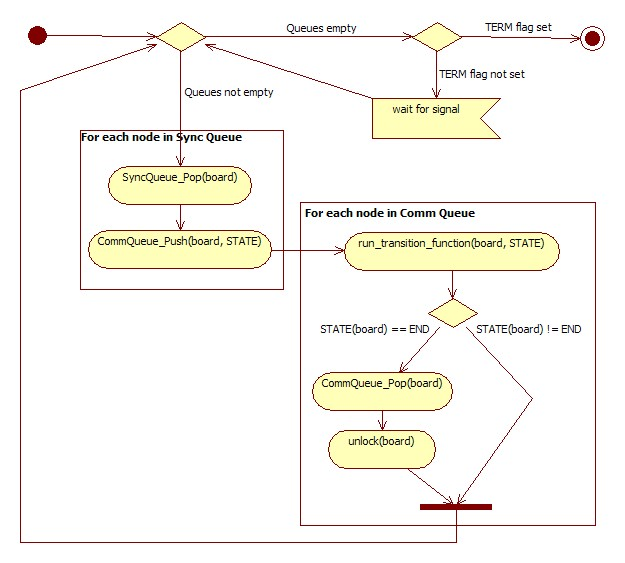
\includegraphics[scale=0.50]{commloop.jpg}
 \caption{Activity diagram for Communication Thread}
 \label{fig:commloop}
\end{figure}

\begin{figure}[h]
 \centering
  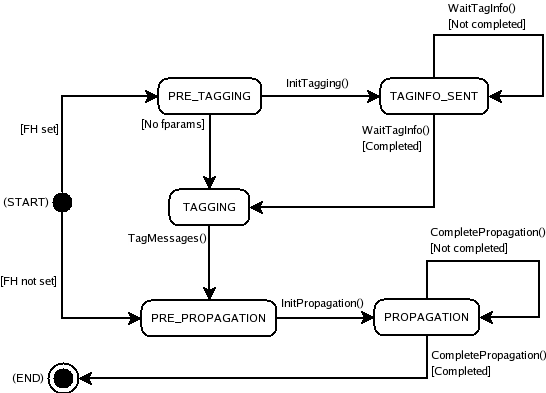
\includegraphics[scale=0.50]{CommNode.png}
 \caption{State diagram for processing Communication Node}
 \label{fig:commstate}
\end{figure}

% ===========================================================================
\subsection{Issues}

\begin{itemize}
\item MPI thread support
\item MPI sends/receives requires contiguous buffers. Expensive (space and time) packing of messages.
\item Comm stages not fully non-blocking
\item Total tagged messages may be more than actual message. Gets works with more proc. Scaling issues.
\end{itemize} 

% ===========================================================================
